\label{5_resultados}

\section{Parâmetros analisados}

Foram escolhidos parâmetros simples para analisar a evolução feita ao longo das gerações:

\begin{itemize}
	\item Valor mínimo de fitness em um indivíduo;
	\item Valor máximo de fitness em um indivíduo;
	\item Valor médio de fitness entre todos os indivíduos;
	\item Desvio padrão dos valores de fitness.
\end{itemize}

O desvio padrão aqui foi calculado por:

\begin{equation}
	\sigma = \sqrt{\frac{1}{N-1} \sum_{i=1}^N (x_i - \overline{x})^2}
\end{equation}

\section{OneMax Booleano}

\begin{figure}[ht!]
    \centering 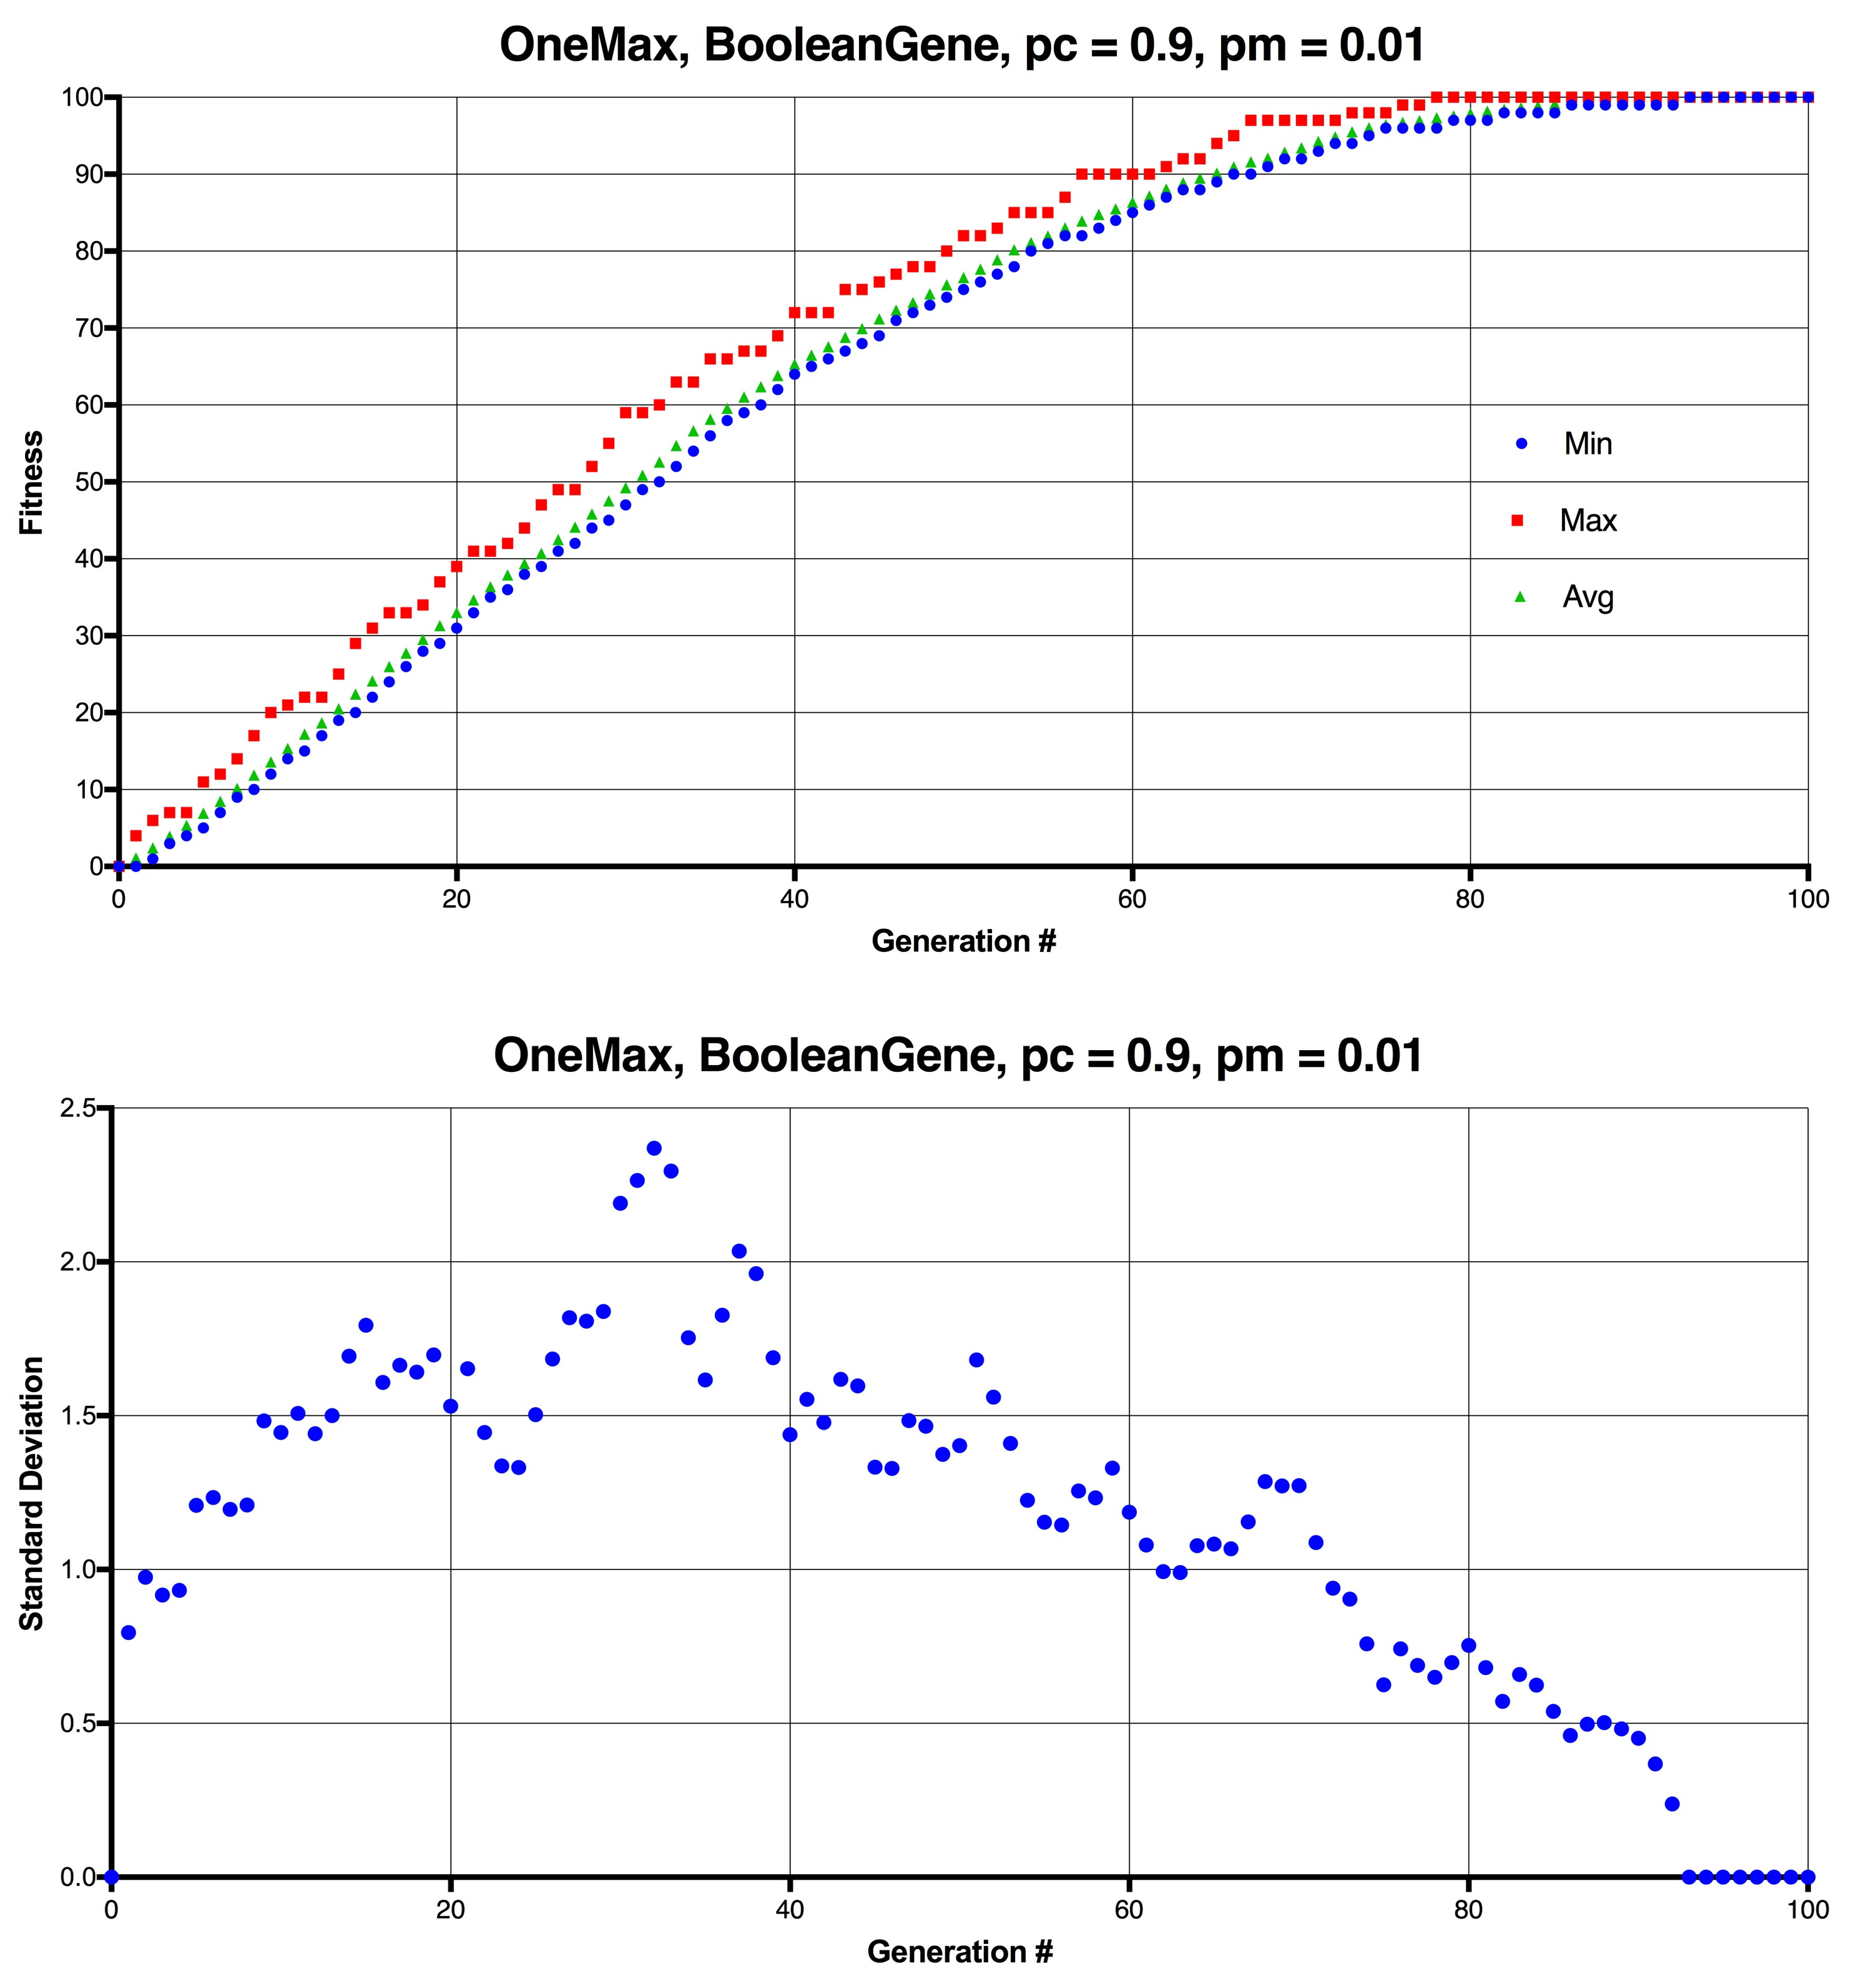
\includegraphics[width=1.0\textwidth]{onemax_boolean.jpg}
    \caption{Evolução do fitness para o problema do OneMax Booleano com mínimo, máximo e valor médio, com $p_c=0.9$ e $p_m=0.01$.}
    \label{fig:onemax_boolean}
\end{figure}

\begin{figure}[ht!]
    \centering 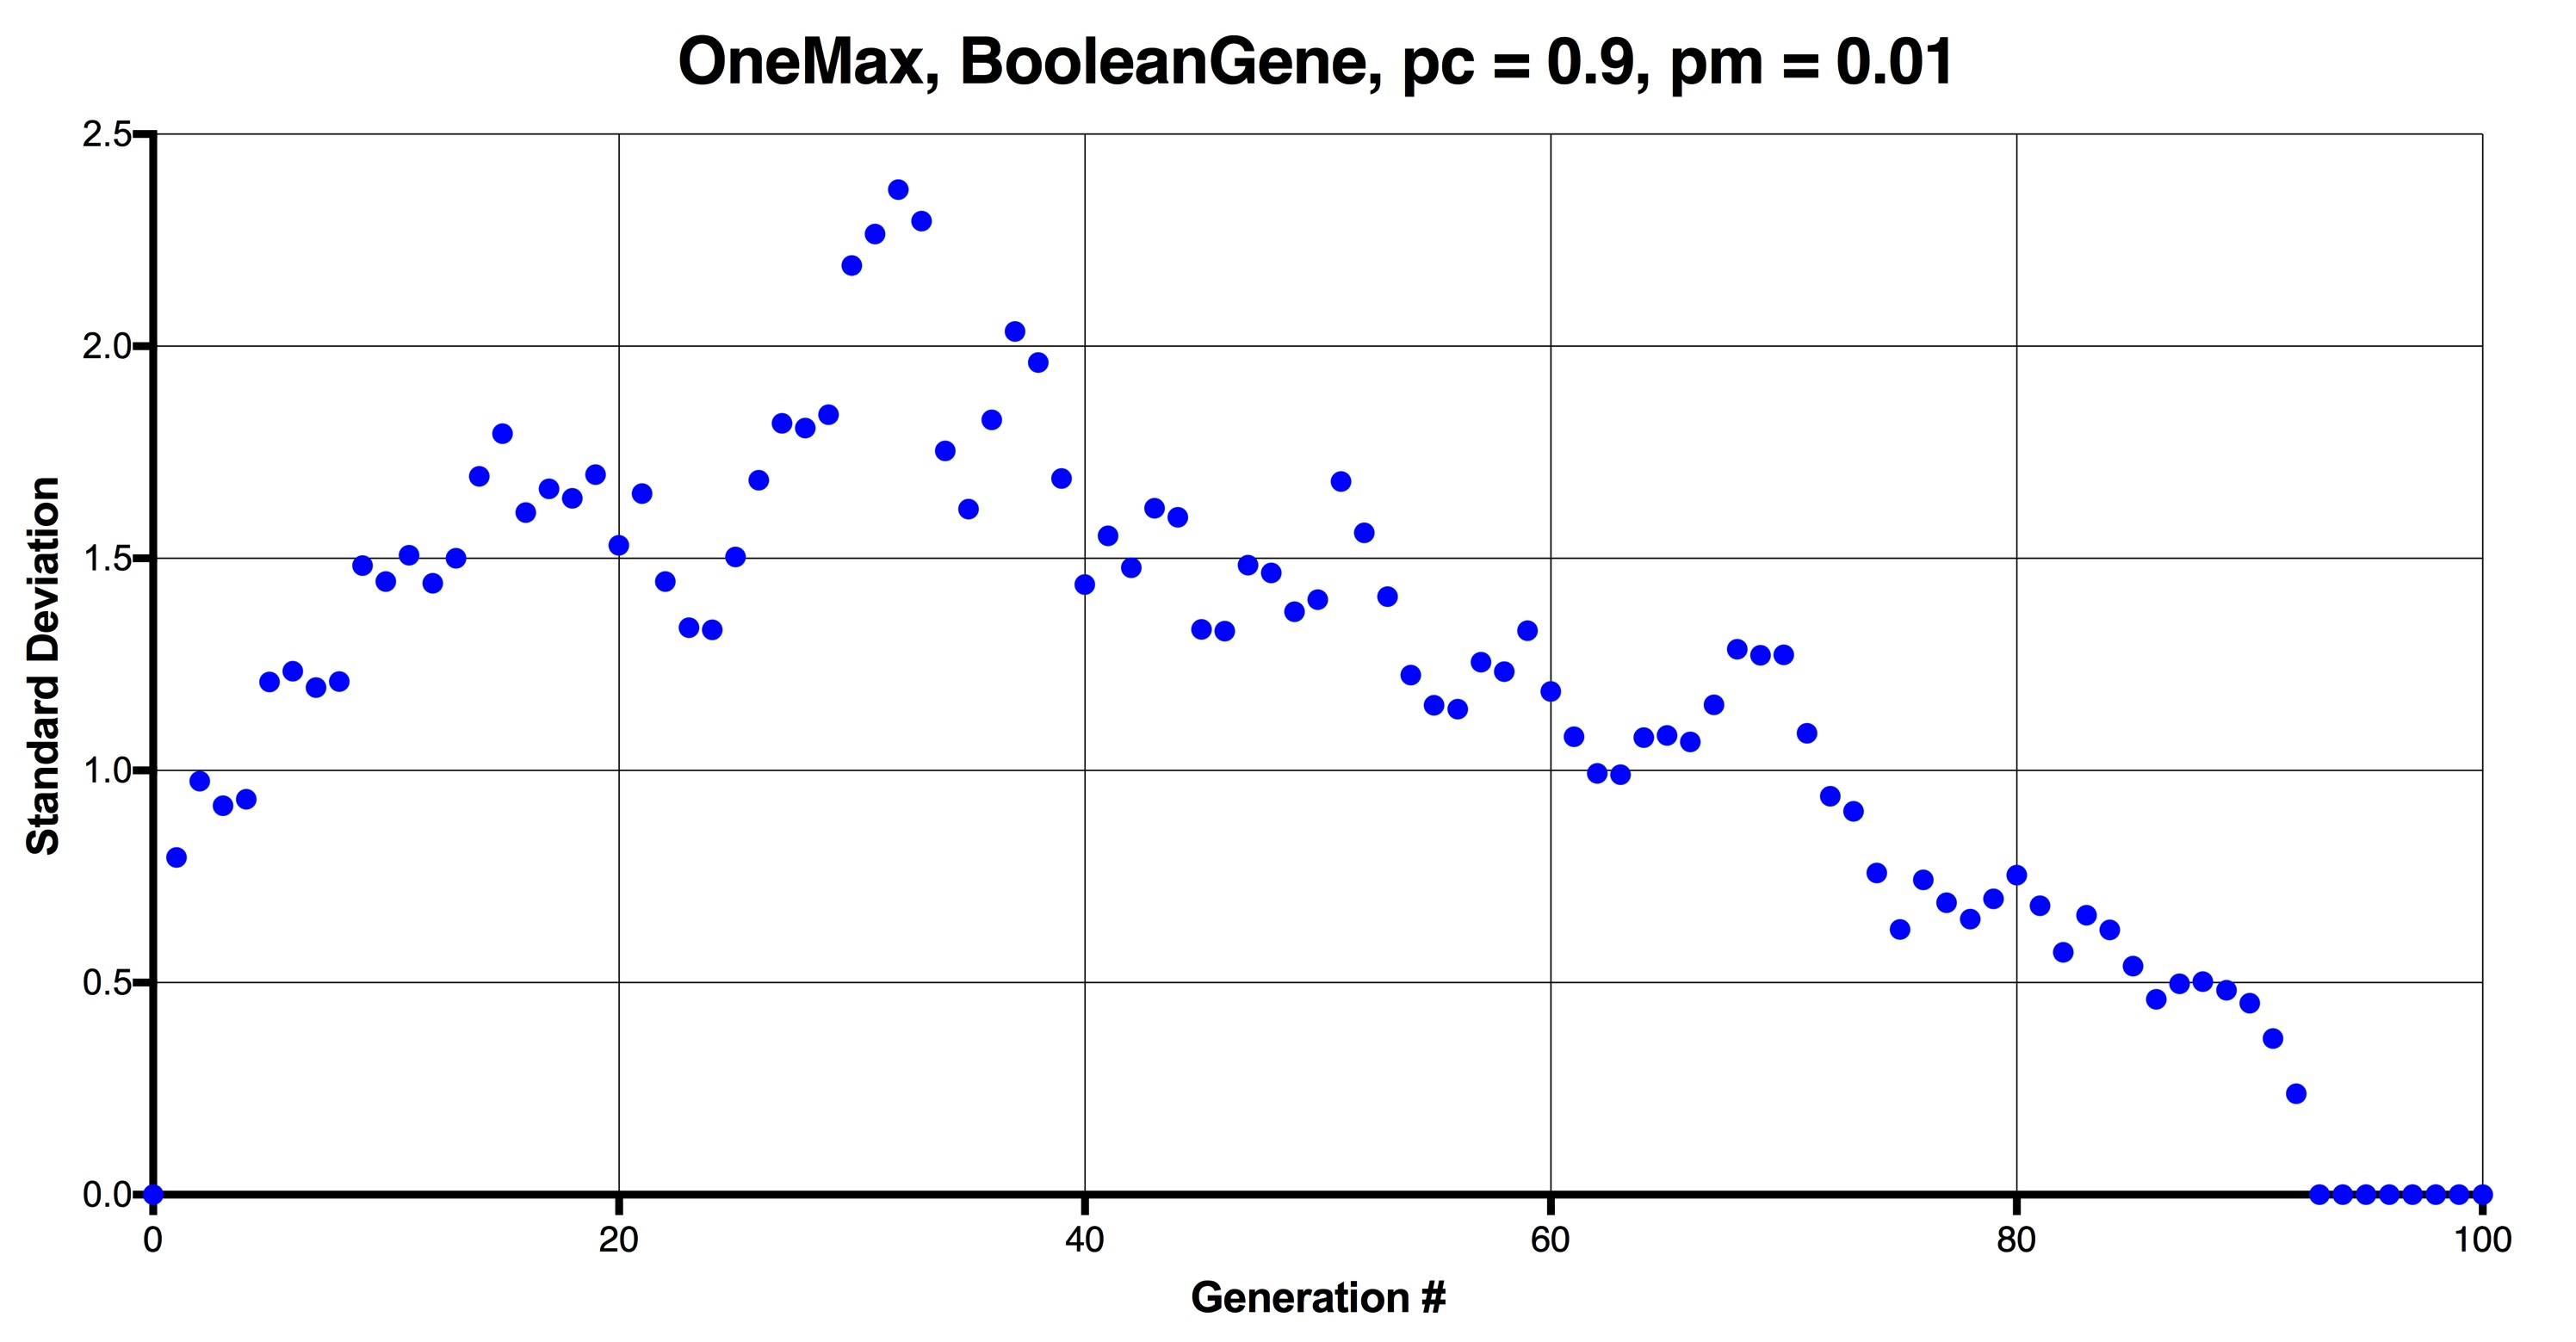
\includegraphics[width=1.0\textwidth]{onemax_boolean_std.jpg}
    \caption{Desvio padrão ao longo das gerações para o problema do OneMax Booleano, com $p_c=0.9$ e $p_m=0.01$.}
    \label{fig:onemax_boolean}
\end{figure}

\section{OneMax Real}

\begin{figure}[ht!]
    \centering 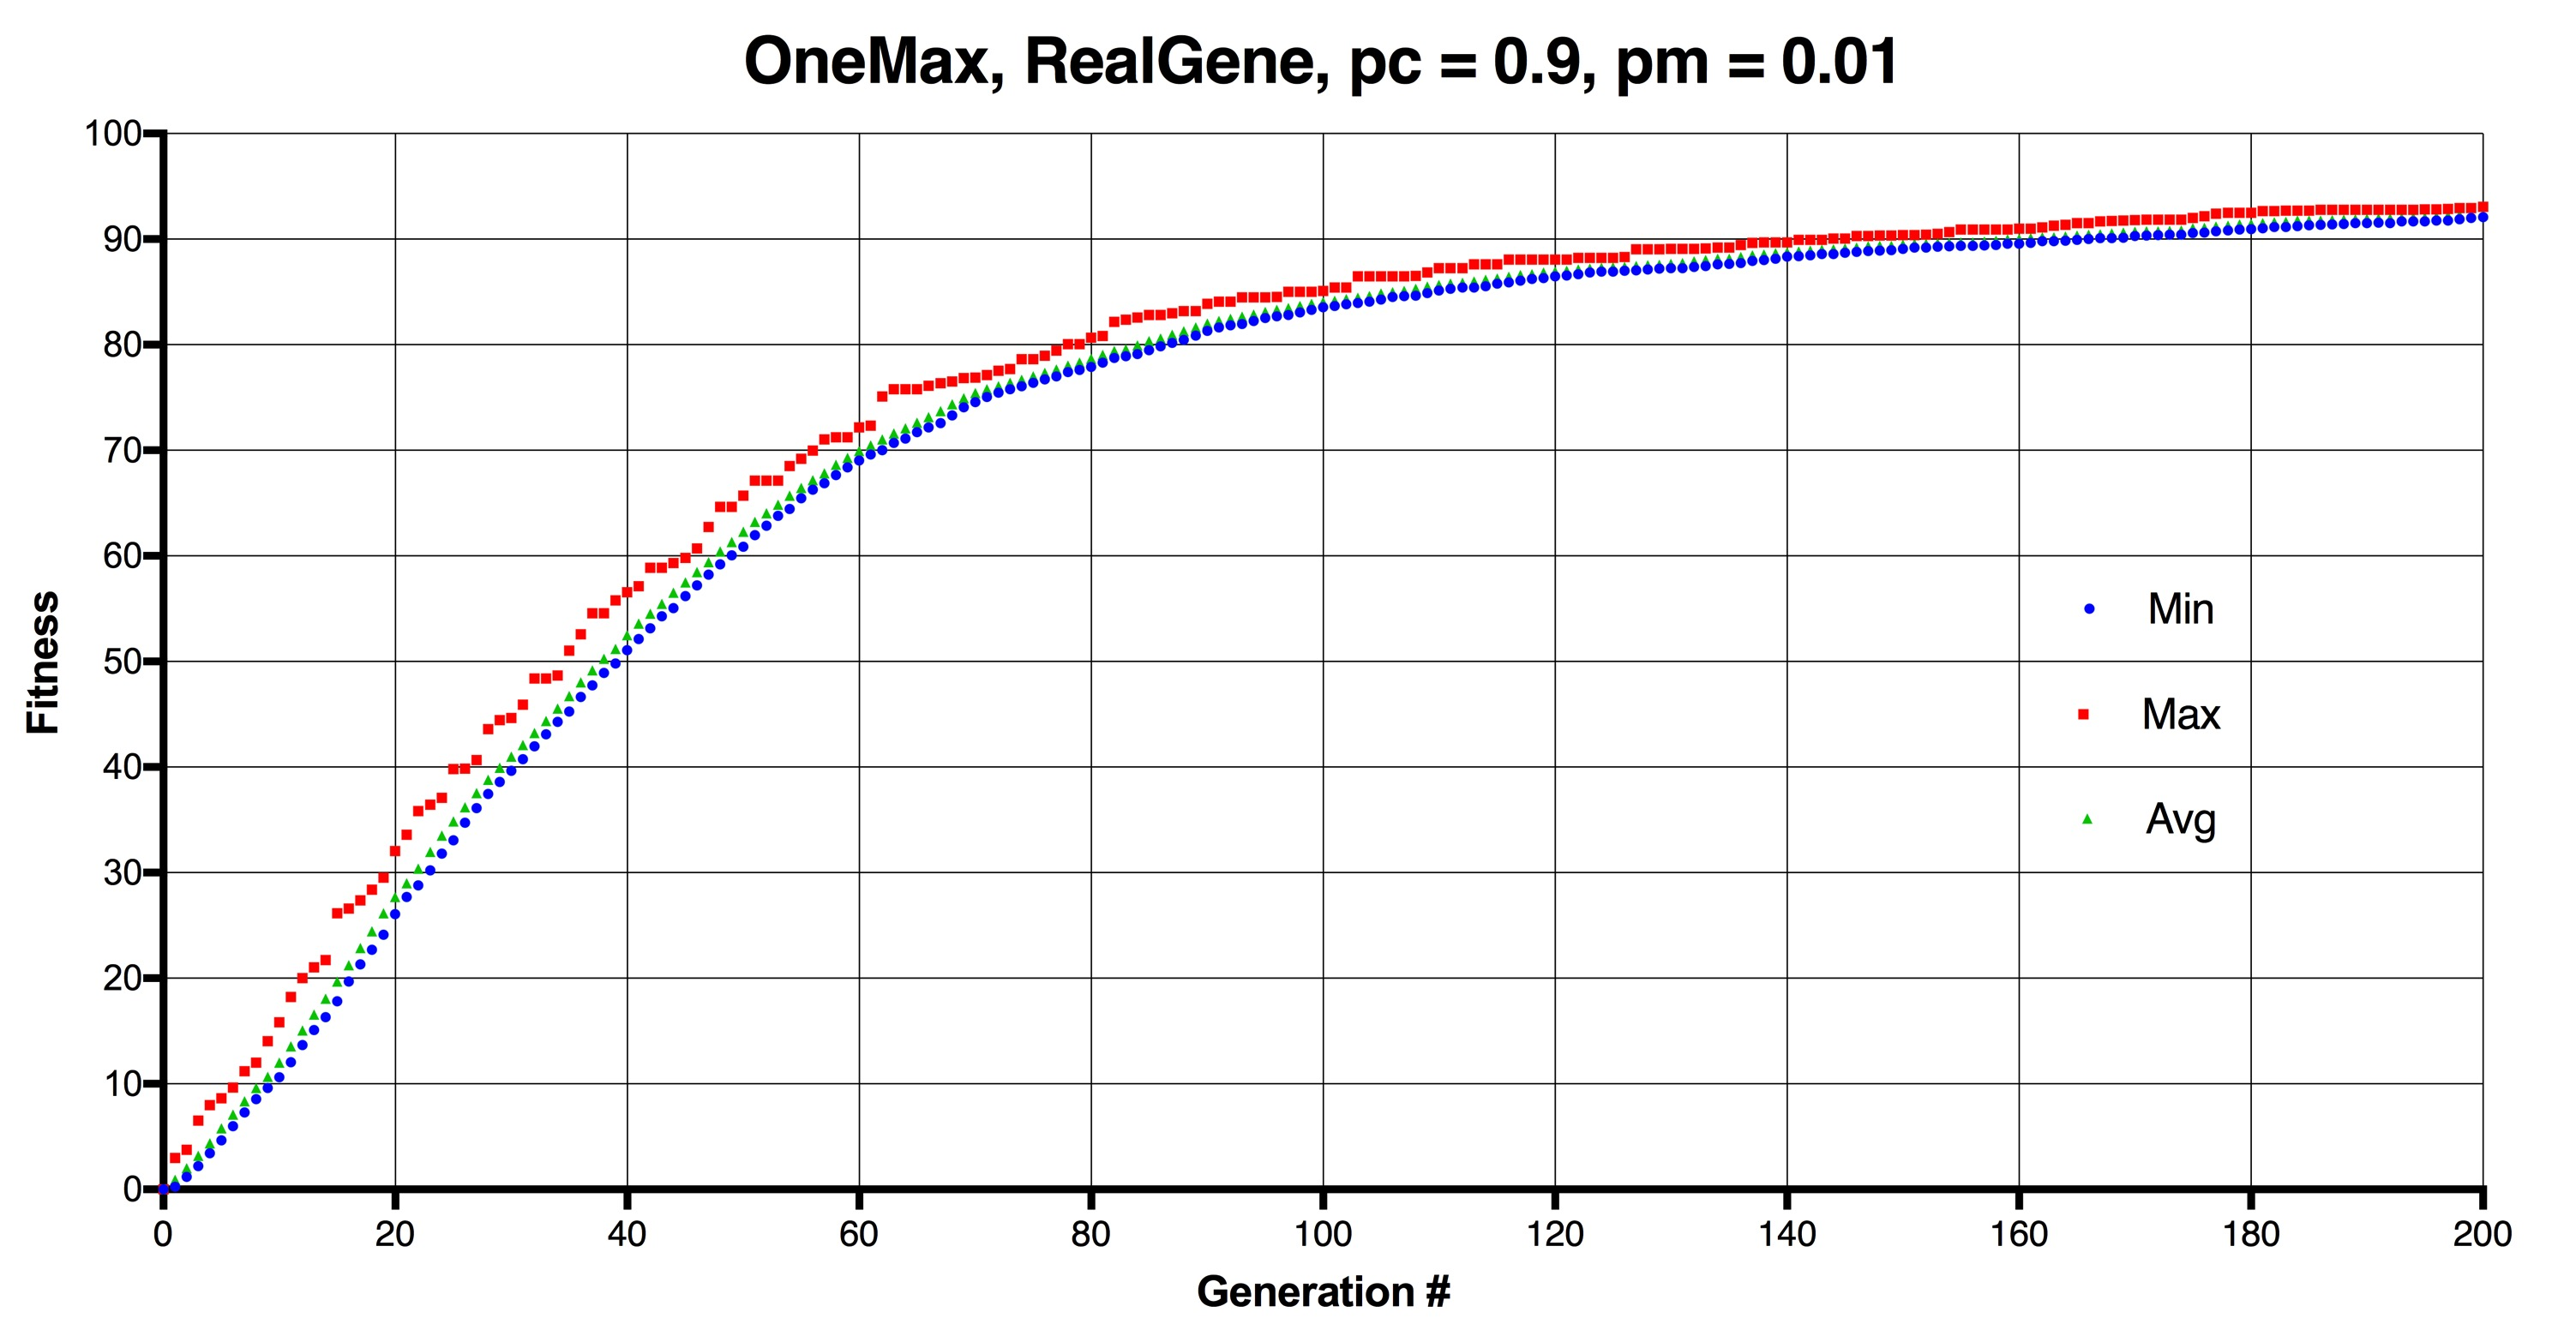
\includegraphics[width=1.0\textwidth]{onemax_real.jpg}
    \caption{Evolução do fitness para o problema do OneMax Real com mínimo, máximo e valor médio, com $p_c=0.9$ e $p_m=0.01$.}
    \label{fig:onemax_boolean}
\end{figure}

\begin{figure}[ht!]
    \centering 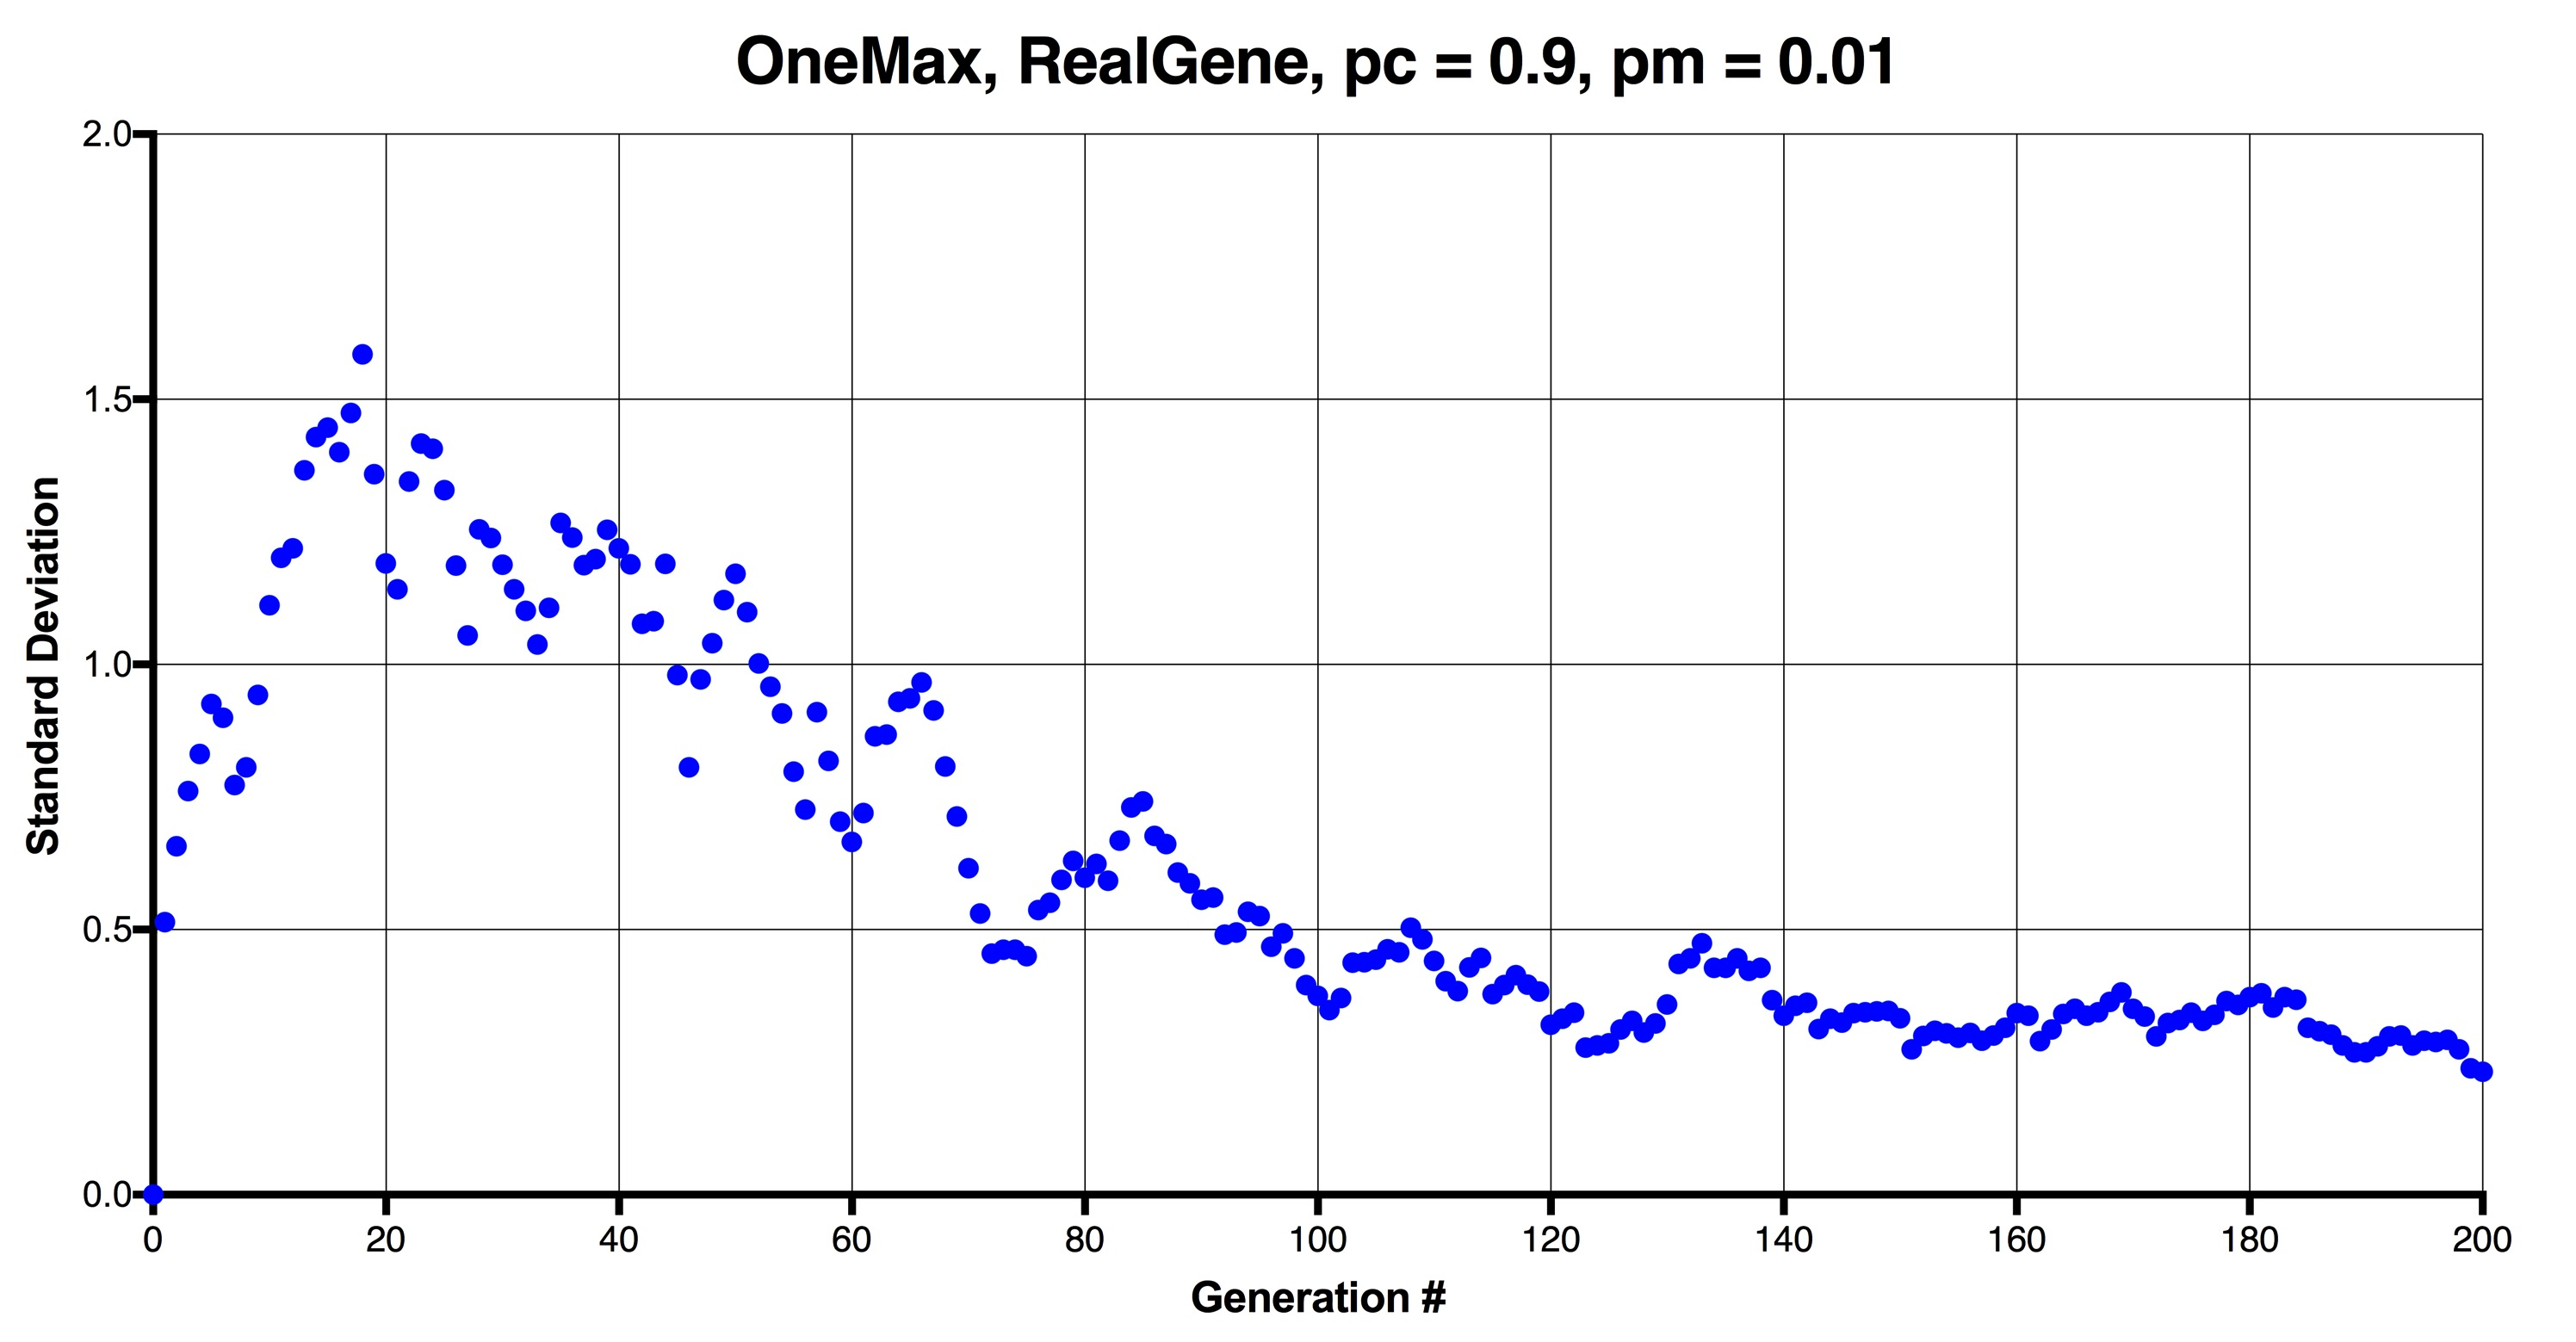
\includegraphics[width=1.0\textwidth]{onemax_real_std.jpg}
    \caption{Desvio padrão ao longo das gerações para o problema do OneMax Real, com $p_c=0.9$ e $p_m=0.01$.}
    \label{fig:onemax_boolean}
\end{figure}

Texto aqui.